\documentclass[11pt]{article}

%-----------Packeges---------------%
\usepackage{amsmath}
\usepackage{amssymb}
\usepackage{amsfonts}
\usepackage{tocloft}
\usepackage{float}
\usepackage{graphicx}
\usepackage[bookmarks=true]{hyperref}
\usepackage{fancyhdr}


%----------Definition & Theorem----%
\newtheorem{definition}{Definition}[subsection]
\newtheorem{theorem}{Theorem}[subsection]
\newtheorem{proposition}{Proposition}[subsection]
\newtheorem{lemma}{Lemma}[subsection]
\newtheorem{corollary}{Corollary}[subsection]

\usepackage{listings}
\pagestyle{fancy}
\fancyhead[L]{Math 417}
\fancyhead[C]{HW5}
\fancyhead[R]{Lanxiao Bai(lbai5)}

\begin{document}
\paragraph{2.1.5}
	\subparagraph{Claim:}The group form by $\mathbb{Z}_4$ under addition $C_4$ and the group form by the symmetries of rectangle under the composition of symmetries $K_4$ are not isomorphic.
	\subparagraph{Proof:}
		The multiplication tables of each group are as the following:
		\begin{table}[!hbp]
			\centering
			\begin{tabular}{c || c | c | c | c }
			 $+$ & $[0]$ & $[1]$ & $[2]$ & $[3]$\\
			 \hline
			 $[0]$ & $[0]$ & $[1]$ & $[2]$ & $[3]$\\
			 \hline
			 $[1]$ & $[1]$ & $[2]$ & $[3]$ & $[0]$\\
			 \hline
			 $[2]$ & $[2]$ & $[3]$ & $[0]$ & $[1]$\\
			 \hline
			 $[3]$ & $[3]$ & $[0]$ & $[1]$ & $[2]$\\
			 \hline
			\end{tabular}
			\caption{Multiplication Table of $C_4$}
		\end{table} 
		\begin{table}[!hbp]
			\centering
			\begin{tabular}{c || c | c | c | c }
			 $\cdot$ & $e$ & $r_1$ & $r_2$ & $r_3$\\
			 \hline
			 $e$ & $e$ & $r_1$ & $r_2$ & $r_3$\\
			 \hline
			 $r_1$ & $r_1$ & $e$ & $r_3$ & $r_2$\\
			 \hline
			 $r_2$ & $r_2$ & $r_3$ & $e$ & $r_1$\\
			 \hline
			 $r_3$ & $r_3$ & $r_2$ & $r_1$ & $e$\\
			 \hline
			\end{tabular}
			\caption{Multiplication Table of $K_4$}
		\end{table}
		
		And their Cayley graphs can show the differences more clearly.
		
	\begin{figure}[H]
        \begin{center}
        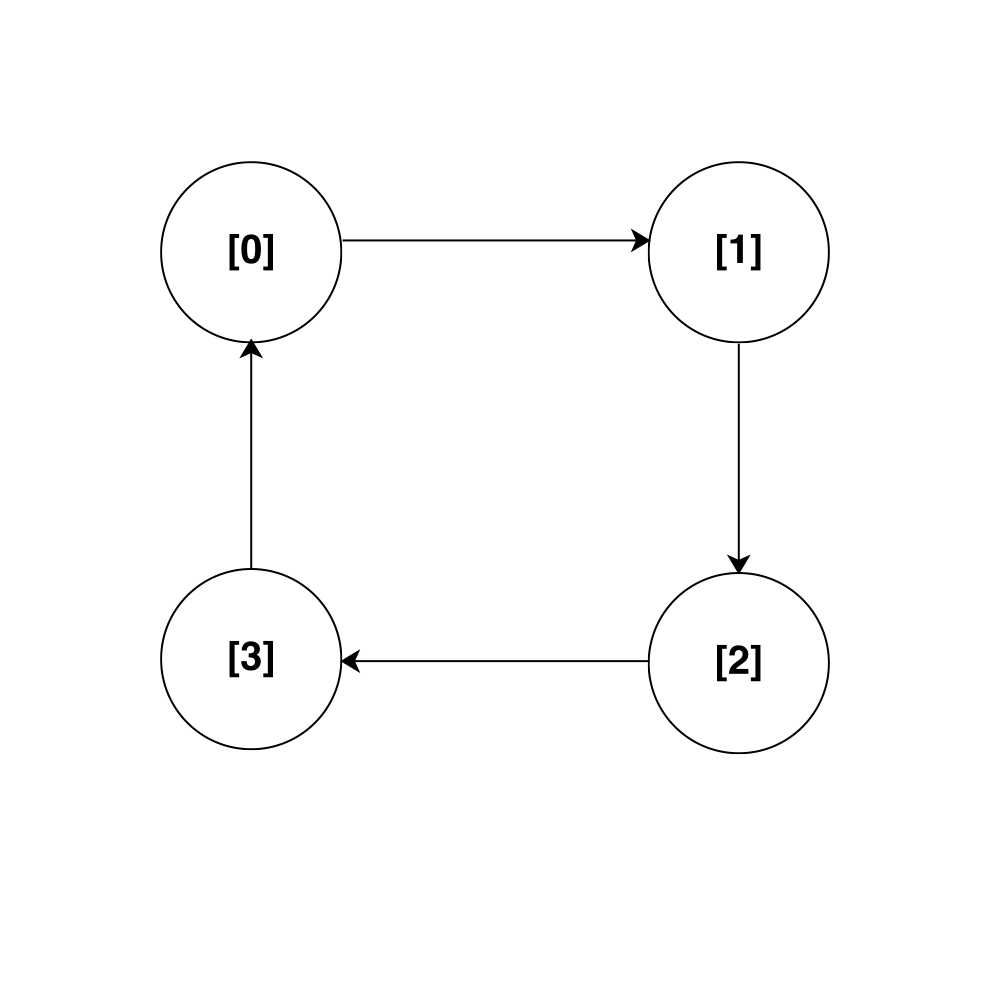
\includegraphics[width=5cm]{./imgs/C_4.png}
        \caption{Cayley Graph of $C_4$}
        \end{center}
    \end{figure}
    
    \begin{figure}[H]
        \begin{center}
        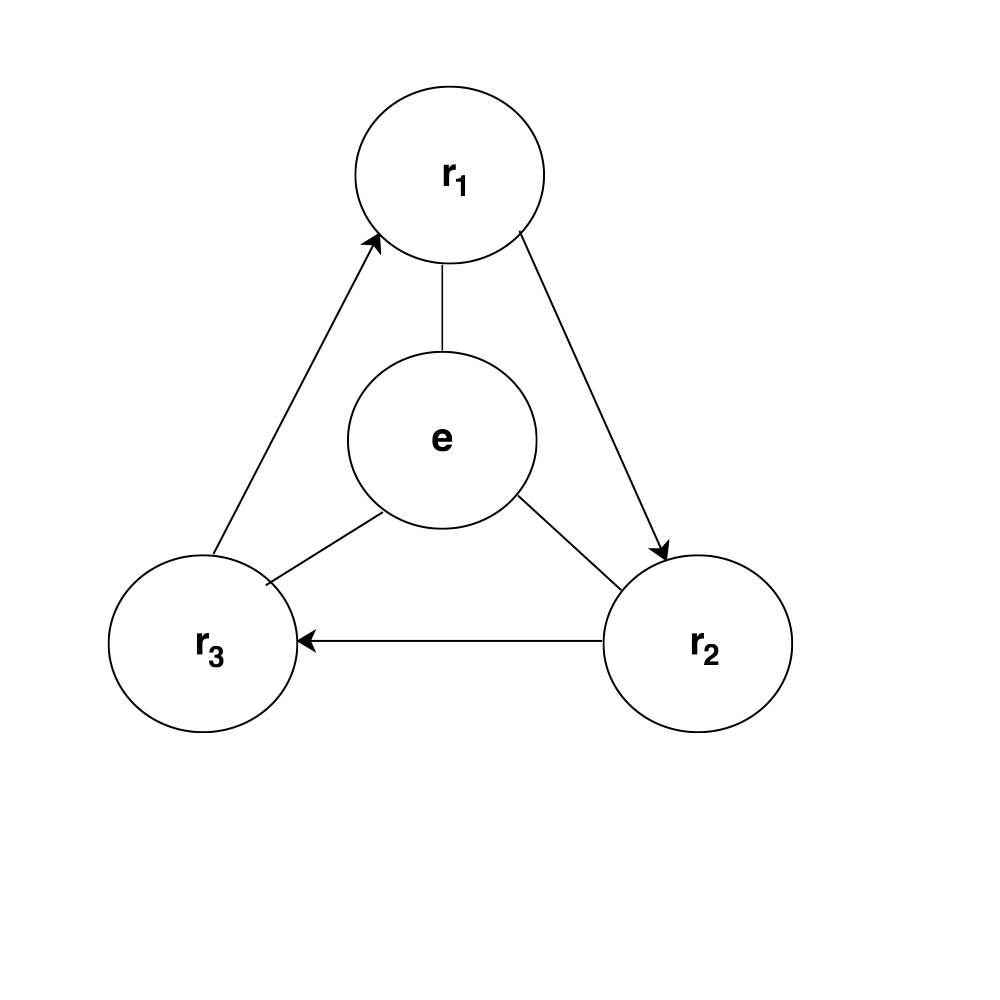
\includegraphics[width=5cm]{./imgs/K_4.png}
        \caption{Cayley Graph of $K_4$}
        \end{center}
    \end{figure}
		
	So we can conclude that The group form by $\mathbb{Z}_4$ under addition $C_4$ and the group form by the symmetries of rectangle under the composition of symmetries $K_4$ are not isomorphic.$\blacksquare$
\paragraph{2.1.15}
	\subparagraph{Claim:} The following mathematical statements are equivalent for a group $G$:
			\begin{enumerate}
				\item $G$ is abelian
				\item $\forall a,b \in G, (ab)^{-1} = a^{-1}b^{-1}$
				\item $\forall a,b \in G, aba^{-1}b^{-1} = e$
				\item $\forall a,b \in G, (ab)^{2} = a^{2}b^{2}$
				\item $\forall a,b \in G, n \in \mathbb{N}, (ab)^{n} = a^{n}b^{n}$
			\end{enumerate}
			
			\subparagraph{Proof:}
				To prove all those statements are equivalent, we can prove that $1 \Rightarrow 2 \Rightarrow 3 \Rightarrow 4 \Rightarrow 5 \Rightarrow 1$. So we can prove them separately.\\
				
				\textbf{$1 \Rightarrow 2$: } Since $G$ is an abelian group, so $\forall a, b \in G, ab = ba$.
				
				Then since $(ab)^{-1} = b^{-1}a^{-1}$ and $b^{-1}a^{-1} = a^{-1}b^{-1}$, so $(ab)^{-1} = a^{-1}b^{-1}$ is proved.\\
				
				\textbf{$2 \Rightarrow 3$: } $aba^{-1}b^{-1} = ab(a^{-1}b^{-1}) = (ab)(ab)^{-1} = e$.\\
				
				\textbf{$3 \Rightarrow 4$: }$(ab)^2 = (ab)(ab)$. Since $aba^{-1}b^{-1} = e$, $aba^{-1}b^{-1}ba = ba \Leftrightarrow ab = ba$, so $(ab)(ab) = (ab)(ba) = a(bb)a = ab^2a = aab^2 = a^2b^2$.\\
				
				\textbf{$4 \Rightarrow 5$: }Since $(ab)^2 = a^2b^2$, $(ab)^2(ab)^{-1} =  a^2b^2(ab)^{-1} \Leftrightarrow ab = a^2b^2b^{-1}a^{-1} = a^2ba^{-1} \Leftrightarrow a^{-1}aba = a^{-1}a^2ba^{-1}a \Leftrightarrow ba = ab$.
				
				Then we can use mathematical induction to prove this statement.
				
				Base case: when $n = 1$, $ab = ab$ is obvious.
				
				Suppose that when $n = k$, we have $(ab)^k = a^kb^k$, then if $n = k + 1$, $(ab)^{k + 1} = (ab)^k \cdot (ab) = a^kb^k(ab) = a^kb^k(ba) = a^k(b^kb)a = a^kb^{k + 1}a = a^kab^{k + 1} = a^{k + 1}b^{k + 1}$.
				
				So we can conclude that $\forall a,b \in G, n \in \mathbb{N}, (ab)^{n} = a^{n}b^{n}$.\\
				
				 \textbf{$5 \Rightarrow 1$: }Since $\forall a,b \in G, n \in \mathbb{N}, (ab)^{n} = a^{n}b^{n}$, let $n = 2$, then $(ab)^2 = a^2b^2$. So $(ab)^2 = a^2b^2$, $(ab)^2(ab)^{-1} =  a^2b^2(ab)^{-1} \Leftrightarrow ab = a^2b^2b^{-1}a^{-1} = a^2ba^{-1} \Leftrightarrow a^{-1}aba = a^{-1}a^2ba^{-1}a \Leftrightarrow ba = ab$.\\
				 
				Thus, we can finally conclude that the  mathematical statements above are equivalent for a group $G$.$\blacksquare$
\paragraph{2.2.2}\textbf{Solution:}
	\begin{figure}[H]
        \begin{center}
        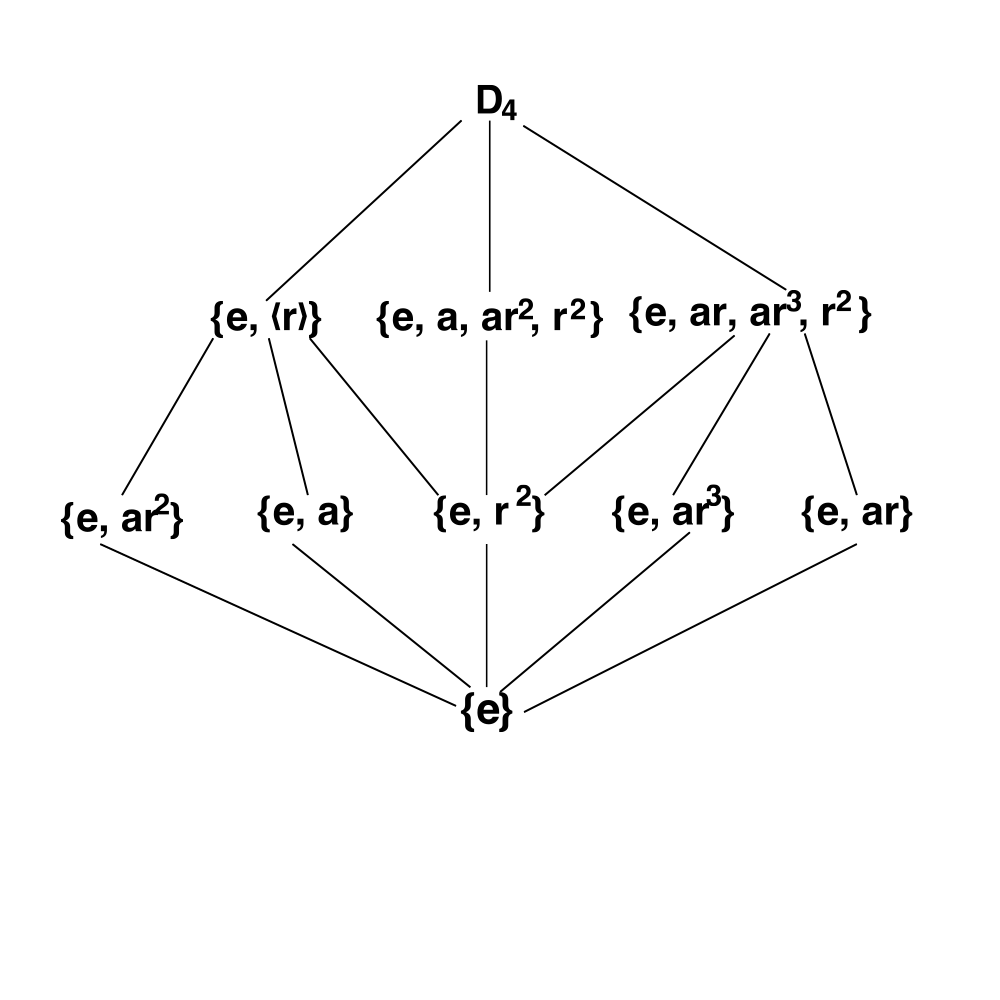
\includegraphics[width=6cm]{./imgs/D_4.png}
        \caption{Subgroup Lattice of $D_4$}
        \end{center}
    \end{figure}
	
\paragraph{2.2.7}
	\subparagraph{Claim:} If $H_1, H_2, \cdots, H_n$ are subgroups of $G$, then $\bigcap_{\alpha}H_{\alpha}$ is s subgroup of $G$.
	\subparagraph{Proof:}
		 We can use induction to prove that $\forall n \in \mathbb{N}$, we have $\bigcap_{\alpha}H_{\alpha}$ is s subgroup of $G$.
		 
		 Base case, when $n = 1$, if $H_1$ is a subgroup of $G$, $\bigcap_{i = 1}^1H_{i} = H_1$ is a subgroup of $G$ is obviously true.
		 
		 Suppose that when $n = k$, $\bigcap_{i = 1}^kH_{i}$. Then if $n = k + 1$, $\bigcap_{i = 1}^{k + 1}H_{i} = (\bigcap_{i = 1}^{k}H_{i}) \bigcap H_{k + 1}$ while $\bigcap_{i = 1}^{k}H_{i}$ and $H_{k+1}$ are both subgroups of $G$.
		 
		 If $\bigcap_{i = 1}^{k}H_{i} \subseteq H_{k+1}$ or $H_{k+1} \subseteq \bigcap_{i = 1}^{k}H_{i}$, then $\bigcap_{i = 1}^{k + 1}H_{i} = H_{k+1}$ or $\bigcap_{i = 1}^{k}H_{i}$. According to base case, $\bigcap_{i = 1}^{k + 1}H_{i} = H_{k+1}$ is a subgroup of $G$.
		 
		 If $\bigcap_{i = 1}^{k}H_{i} \nsubseteq H_{k+1}$ or $H_{k+1} \nsubseteq \bigcap_{i = 1}^{k}H_{i}$ and $\bigcap_{i = 1}^{k + 1}H_{i} \neq \emptyset$, since for all i, $e \in H_i$, $e \in \bigcap_{i = 1}^{k + 1}H_{i}$. Take $g \in \bigcap_{i = 1}^{k + 1}H_{i}$, then for all i, $g \in H_i$. Since each $H_i$ is a subgroup, $g^{-1} \in H_i$ for each i, thus $g^{-1} \in \bigcap_{i = 1}^{k + 1}H_{i}$. Take $g, h \in H$. Then $g, h \in H_i$ for every $i$, so $gh \in H_i$ for every i. Thus $gh \in H$.
		 
		 So we can conclude that If $H_1, H_2, \cdots, H_n$ are subgroups of $G$, then $\bigcap_{\alpha}H_{\alpha}$ is s subgroup of $G$.$\blacksquare$
		
\paragraph{2.2.24}
	\subparagraph{Claim:} If there's at least $3$ elements of order $4$, the group of order $20$ cannot be cyclic. If there's exactly $2$ element of order $4$, the group of order $20$ can be cyclic.
	\subparagraph{Proof:} Suppose the group $G$ of order 20 has at least $3$ elements of order $4$ is cyclic. That is to say that $G \cong C_{20} \cong \mathbb{Z}_{20}$. Since there're only $20$ elements in $\mathbb{Z}_{20}$, we can check all elements if they are element of order $4$. 
	
	By definition, if $[i] \in \mathbb{Z}_{20}$ is an order $4$ element, it is expected that $(4 \cdot x) \mod 20 = 0$ and for $i = 1, 2 ,3$, $(i \cdot x) \mod 20 \neq 0$. Since it's tiring to calculate all $20$ elements, so I wrote some code to do this for me as the following with Python 2.7.10(next page).
	
	\begin{figure}[H]
        \begin{center}
        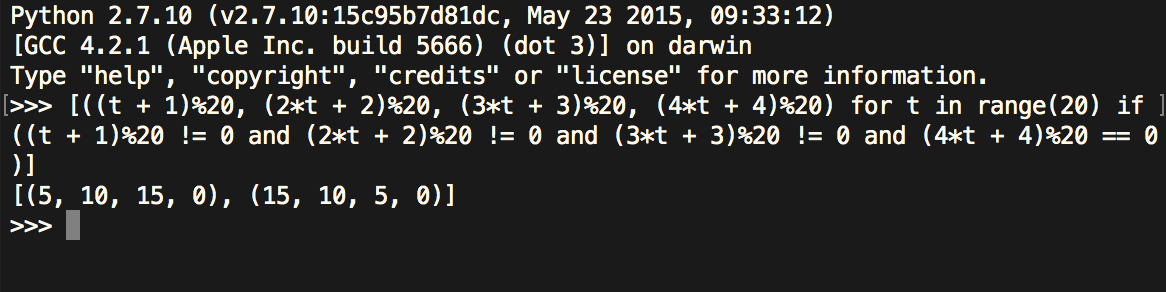
\includegraphics[width=10cm]{./imgs/code.png}
        \caption{Python Code}
        \end{center}
    \end{figure}
    
    As the code shows, there's only $2$ elements of order $4$ in $C_{20}$. 
    
    As a result, we proved that, if there's at least $3$ elements of order $4$, the group of order $20$ cannot be cyclic. If there's exactly $2$ element of order $4$, the group of order $20$ can be cyclic.$\blacksquare$
		
\end{document}
